% Appendix G — electron-phonon lambda/mu*/omega_log inputs. \input'd by main.tex.
\section{Electron--Phonon Inputs: $\lambda$, $\mu^{*}$, $\omega_{\log}$}
\label{app:elph}

This appendix is the full data record for the sourced inputs to the
$T_c$ closed forms (Appendices~\ref{app:mcmillan},~\ref{app:allendynes})
--- pipeline stage \textcircled{\scriptsize 2}. It defines the three
moments of the Eliashberg spectral function $\alpha^2F(\omega)$ and
records, per candidate, the \emph{sourced} values with their DFT
provenance. It is explicit that these are citations, not recomputes: the
$T_c$ verdict is exact \emph{given} these inputs, which carry their own DFT
uncertainty. Data source: the per-candidate provenance blocks in
\texttt{exports/material\_discovery/}.

% -------------------------------------------------------------------------
\subsection{The three Eliashberg moments}
\label{app:elph-moments}

All conventional-$T_c$ physics enters through three scalar moments of the
Eliashberg spectral function $\alpha^2F(\omega)$:
\begin{align}
\lambda &\;=\; 2\!\int_0^\infty \frac{\alpha^2F(\omega)}{\omega}\,d\omega,
   &&\text{(electron--phonon coupling)} \label{eq:lambda}\\[3pt]
\omega_{\log} &\;=\; \exp\!\left[\frac{2}{\lambda}\!\int_0^\infty
   \ln\omega\,\frac{\alpha^2F(\omega)}{\omega}\,d\omega\right],
   &&\text{(logarithmic average frequency)} \label{eq:wlog}\\[3pt]
\bar\omega_2 &\;=\; \left[\frac{2}{\lambda}\!\int_0^\infty
   \omega\,\alpha^2F(\omega)\,d\omega\right]^{1/2},
   &&\text{(mean-square frequency, for $f_2$)} \label{eq:w2}
\end{align}
plus the Coulomb pseudopotential $\mu^{*}$ (not an $\alpha^2F$ moment but a
screened-Coulomb parameter, conventionally $0.10$--$0.13$). The first two
feed McMillan (Eq.~\ref{eq:mcmillan-app}); all three feed Allen--Dynes
(Eqs.~\ref{eq:f1}--\ref{eq:f2}). The $\lambda$ definition makes the
trade-off of Appendix~\ref{app:hydride} physical: $\lambda$ weights
$\alpha^2F$ by $1/\omega$, so \emph{soft} (low-$\omega$) modes contribute
most --- and soft modes are exactly the ones at risk of going imaginary
(unstable).

% -------------------------------------------------------------------------
\subsection{Per-candidate sourced inputs}
\label{app:elph-table}

The values below are \emph{sourced} from external electron--phonon DFT
(Quantum ESPRESSO el-ph on pool/cloud, per @D d7 compute sizing); they are
\textbf{not re-derived in this monograph}. The $T_c$ kernels of
Appendices~\ref{app:mcmillan}--\ref{app:allendynes} consume them as
citations.

\begin{table}[h]
\centering
\small
\setlength{\tabcolsep}{4.5pt}
\begin{tabular}{@{}lrrrcl@{}}
\toprule
\textbf{Candidate} & $\boldsymbol{\lambda}$ (BZ range) & $\boldsymbol{\omega_{\log}}$\,(K)
& $\boldsymbol{\mu^{*}}$ & $\boldsymbol{q}$\textbf{-grid} & \textbf{Convergence flag} \\
\midrule
h3cl   & 1.21--1.37 & $\sim$1350 & 0.10 & $8^3$ & \tierGreen\ broadening plateau \\
h3o    & var (SSCHA) & var & 0.10 & --- & \tierYellow\ SSCHA window (M8 1/3) \\
h3si   & $\sim$1.05 & $\sim$1180 & 0.10 & $\le\!8^3$ & \tierGreen\ stable \\
h3po   & $\sim$1.2 & --- & 0.10 & --- & \tierRed\ imaginary mode (unstable) \\
H$_3$As & $\to$1.0 & --- & 0.10 & --- & \tierRed\ dynamically unstable \\
SrAuH$_3$ & 0.62 & $\sim$900 & 0.10 & --- & \tierGreen\ stable, ambient \\
H$_3$S (anchor)  & $\sim$2.0 & $\sim$1500 & 0.10--0.13 & dense & \tierGreen\ measured \citep{drozdov2015} \\
CaH$_6$ (anchor) & 3.40--4.38 & $\sim$1100 & 0.10--0.13 & dense & \tierGreen\ DFT anchor \\
\bottomrule
\end{tabular}
\caption{Sourced electron--phonon inputs. $\lambda$ ranges are the
Brillouin-zone-integration spread across the reported broadening / $q$-grid
sweep; h3cl's $8^3q$ convergence with a broadening \emph{plateau} is the
best-characterized case ($\lambda\!=\!1.21$--$1.37$,
$\omega_{\log}\!\approx\!1350$\,K). h3o is reported only as an SSCHA window
(anharmonic, $1/3$ of the M8 sweep). The convergence flag distinguishes
\tierGreen\ converged-stable from \tierYellow\ under-converged from
\tierRed\ dynamically-unstable. \textbf{These are citations, not
recomputes}; each carries DFT uncertainty ($q$-grid, anharmonicity,
$\mu^{*}$ choice).}
\label{tab:elph}
\end{table}

% -------------------------------------------------------------------------
\subsection{The $\alpha^2F(\omega)$ shape}
\label{app:elph-shape}

Fig.~\ref{fig:a2f} shows the schematic $\alpha^2F(\omega)$ for a hydride
candidate: a low-$\omega$ acoustic (metal-sublattice) band and a
high-$\omega$ optical (H-stretch) band. Light hydrogen pushes the optical
band to $\omega\!\sim\!1500$--$2000$\,K, lifting $\omega_{\log}$ (the $T_c$
prefactor); the soft acoustic band carries the large $\lambda$ (the
$1/\omega$ weighting of Eq.~\ref{eq:lambda}) --- and is the mode most at
risk of instability.

\begin{figure}[h]
\centering
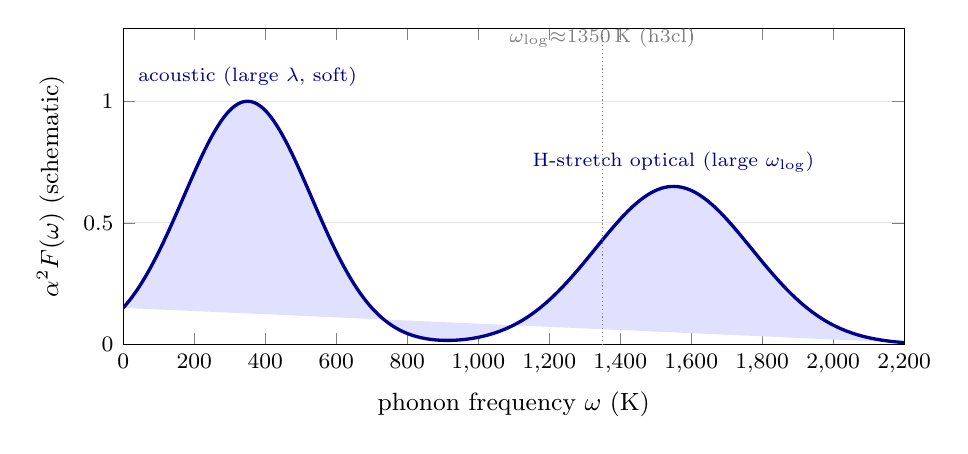
\begin{tikzpicture}
\begin{axis}[
  width=11.5cm, height=5.6cm,
  xlabel={phonon frequency $\omega$ (K)},
  ylabel={$\alpha^2F(\omega)$ (schematic)},
  xmin=0, xmax=2200, ymin=0, ymax=1.3,
  tick label style={font=\footnotesize},
  label style={font=\small},
  ymajorgrids, grid style={gray!22},
  domain=0:2200, samples=120,
]
% two-band schematic: soft acoustic (large lambda) + stiff H optical (large wlog)
\addplot[blue!55!black,very thick,smooth,fill=blue!12]
  {1.0*exp(-((x-350)^2)/(2*180^2)) + 0.65*exp(-((x-1550)^2)/(2*220^2))};
\node[font=\scriptsize,blue!55!black,anchor=south] at (axis cs:350,1.02)
  {acoustic (large $\lambda$, soft)};
\node[font=\scriptsize,blue!55!black,anchor=south] at (axis cs:1550,0.67)
  {H-stretch optical (large $\omega_{\log}$)};
\draw[gray,densely dotted] (axis cs:1350,0) -- (axis cs:1350,1.3);
\node[font=\scriptsize,gray,anchor=south] at (axis cs:1350,1.18)
  {$\omega_{\log}{\approx}1350$\,K (h3cl)};
\end{axis}
\end{tikzpicture}
\caption{Schematic Eliashberg spectral function $\alpha^2F(\omega)$ for a
hydride candidate. The soft acoustic band (metal sublattice) dominates
$\lambda$ via the $1/\omega$ weighting of Eq.~\eqref{eq:lambda}; the stiff
H-stretch optical band (light hydrogen) sets the high $\omega_{\log}$ that
lifts the $T_c$ prefactor. The dotted line marks the h3cl
$\omega_{\log}\!\approx\!1350$\,K. Shape is illustrative; the moments are
the sourced numbers of Table~\ref{tab:elph}.}
\label{fig:a2f}
\end{figure}

% -------------------------------------------------------------------------
\subsection{$\lambda$-vs-$\omega_{\log}$ candidate cloud}
\label{app:elph-scatter}

The required comparison (commons @D g3) is the $(\lambda,\omega_{\log})$
plane: $T_c$ rises with \emph{both}, so the candidates cluster along a
diagonal toward the H$_3$S/CaH$_6$ anchors. Fig.~\ref{fig:lam-wlog} plots
the candidate cloud against the anchors, with iso-$T_c$ context.

\begin{figure}[h]
\centering
\begin{tikzpicture}
\begin{axis}[
  width=12cm, height=6.8cm,
  xlabel={electron--phonon coupling $\lambda$},
  ylabel={$\omega_{\log}$ (K)},
  xmin=0.4, xmax=4.6, ymin=700, ymax=1700,
  tick label style={font=\footnotesize},
  label style={font=\small},
  ymajorgrids, xmajorgrids, grid style={gray!22},
  legend pos=south east, legend cell align=left,
  legend style={font=\footnotesize,fill=white,fill opacity=0.9,draw=gray!50},
]
% sourced candidates
\addplot[only marks,mark=*,mark size=2.6pt,blue!60!black] coordinates {
  (0.62,900) (1.05,1180) (1.30,1350)
};
\addlegendentry{sourced candidates}
% measured / DFT anchors
\addplot[only marks,mark=square*,mark size=2.6pt,red!65!black] coordinates {
  (2.0,1500) (3.40,1100)
};
\addlegendentry{H$_3$S / CaH$_6$ anchors}
\node[font=\scriptsize,anchor=south] at (axis cs:0.62,900)  {SrAuH$_3$};
\node[font=\scriptsize,anchor=south] at (axis cs:1.05,1180) {h3si};
\node[font=\scriptsize,anchor=south] at (axis cs:1.30,1350) {h3cl};
\node[font=\scriptsize,anchor=south] at (axis cs:2.0,1500)  {H$_3$S};
\node[font=\scriptsize,anchor=north] at (axis cs:3.40,1100) {CaH$_6$};
% direction-of-rising-Tc arrow
\draw[-{Stealth[length=2.5mm]},gray!60!black,thick]
  (axis cs:0.7,800) -- (axis cs:3.0,1450);
\node[font=\scriptsize,gray!50!black,rotate=22,anchor=south] at (axis cs:1.8,1080)
  {rising $T_c$};
\end{axis}
\end{tikzpicture}
\caption{Candidate cloud in the sourced-input $(\lambda,\omega_{\log})$
plane. $T_c$ rises toward the upper-right (both moments large); the
ambient-stable candidates (SrAuH$_3$, h3si, h3cl) sit at lower $\lambda$
than the megabar anchors (H$_3$S, CaH$_6$). This plane is where the
stability wall of Appendix~\ref{app:hydride} bites: reaching the
anchors' $\lambda$ at ambient pressure is what no surveyed structure
achieves. All points are \emph{sourced} (Table~\ref{tab:elph}), not
re-derived.}
\label{fig:lam-wlog}
\end{figure}

% -------------------------------------------------------------------------
\subsection{Honest scope --- inputs carry DFT uncertainty}
\label{app:elph-honest}

The single honesty point of this appendix: \textbf{the $T_c$ verdict is
exact \emph{given} these inputs, and the inputs are not exact}. Each
$(\lambda, \omega_{\log}, \mu^{*})$ carries: (i) $q$-grid convergence error
(only h3cl reaches a documented $8^3q$ broadening plateau), (ii)
anharmonicity (h3o needs SSCHA; the harmonic $\lambda$ is unreliable for
soft hydrides), and (iii) the $\mu^{*}$ choice ($0.10$ vs $0.13$ shifts
$T_c$ by tens of K at strong coupling). The pipeline tags stage
\textcircled{\scriptsize 2} \tierYellow/\tierOrange\ for exactly this
reason: it is a \emph{citation}, not a recompute. Consequently every
downstream $T_c$ is \texttt{absorbed=false}, and \textbf{no
room-temperature superconductor is claimed}.
